\chapter{Introduction}

In natural language processing, it is frequently necessary to judge the
correctness of sentences generated by some algorithm. For example, a
speech-to-text translator that only recognizes individual words might produce
the following two candidate sentences for the same input audio sample:
\begin{align*}
 \text{He ate soup.} &&
 \text{He aid soup.}
\end{align*}

Both sentences sound the same, but the second candidate sentence should be
discarded because it is syntactically wrong. As another example, a translator
algorithm that translates from another language to English might generate the
following two candidate sentences for some input text:
\begin{align*}
 \text{This is a small red ball.} &&
 \text{This is a red small ball.}
\end{align*}

Both sentences are syntactically correct, but the first sentence should be
preferred because it conforms to the customary rules for adjective ordering in
the English language. Finally, consider a spelling correction process that is
applied to the following sentence: \cite{kukich1992}
\begin{align*}
 \text{The design \textbf{an} construction of the system will take more than a year.}
\end{align*}

Possible replacements for the syntactically wrong word ``an'' include ``a'' and
``and''. In all these situations, a \emph{language model} can be employed to
choose the best result from a set of candidates.
\cite{stolcke2002,youngetal2005} A language model assigns a probability $p_\omega(v)$
to each sentence $v\in\Sigma^*$ (with words from the set $\Sigma$), such that
correct sentences receive a higher probability than incorrect sentences.
\[
 1 > p_\omega\mbig\kla{\text{He ate soup.}} > p_\omega\mbig\kla{\text{He aid soup.}} > p_\omega\mbig\kla{\text{He He He soup.}} > 0
\]

The probability distribution $p_\omega$ is determined by a \emph{model
parameter} $\omega\in\Omega$. The language model describes how to obtain
$p_\omega$ for any $\omega$. $\omega$ is chosen by a suitable \emph{training
algorithm} using a training corpus $c$ containing known good sentences, such
that $\omega$ maximizes the likelihood of this corpus,
\[
 \prod_{v\in c} p_\omega(v).
\]

\section{N-gram models}

One of the simplest language models is the \emph{bigram model}. It interprets
the generation of a sentence as a stochastic process, wherein each word is
chosen with a probability conditional on the word that appeared before it:
\[
 p(\text{He ate soup.}) = b(\text{He}|\#) \cdot b(\text{ate}|\text{He}) \cdot b(\text{soup}|\text{ate}) \cdot b(\#|\text{soup}),
\]
where the model parameter $b$ is a conditional probability distribution of
$\Sigma\cup\brc{\#}$ given $\Sigma\cup\brc{\#}$ and $\#$ is a placeholder word
that stands in for the start and end of the sentence. More generally,
\[
 p(v = v_1\cdots v_n) = b(v_1|\#) \cdot \prod_{i=2}^n b(v_i|v_{i-1}) \cdot b(\#|v_n).
\]
The model parameter $b$ can be chosen by a very simple training algorithm
\cite[pp.~123]{jm09}: Across the corpus, count all bigrams (i.e., all pairs of
words occurring one directly after the other) in the corpus, and also count how
often each word occurs at the start and at the end of a sentence, respectively.
Then set
\[
 b(v|v') = \frac{c(v'v)}{\sum_{v''\in \Sigma\cup\brc{\#}} c(v'v'')}
\]
where $c(v'v)$ is the number of occurrences of the bigram $v'v$ in the corpus.
The normalization ensures that $b$ is a probability distribution.

The bigram model can be generalized to the \emph{N-gram model}, wherein the
next word is chosen with a probability conditional on the $n-1$ words before
it. Training then counts $n$-grams, i.~.e~sequences of $n$ words, hence the
name \emph{N-gram model}. The bigram model is recovered for $n=2$.

Besides the already mentioned applications where language models augment
translators, N-gram models are useful in \emph{augmentive communication}:
Virtual keyboards on smartphones and tablets predict the next word by looking
at the previous $n$ words, thus improving typing speed and accuracy.
\cite{hasan2004n} A similar assistive word prediction system is used by the
physicist Stephen Hawking. \cite{newelletal1998}

\section{Hidden Markov model}

\begin{figure}[t!]
 \label{fig:language-models}
 \caption{Graphic representation of example instances of language models. Left:
 Bigram model, where arrows $v\to v'$ represent a bigram probability
 $b(v'|v)\neq0$.  The start/end marker $\#$ is shown twice to make the diagram
 more readable. Right: Hidden Markov model, with the hidden states ``noun'' and
 ``verb''; adapted from \cite{nel13}. Arrows $q\to q'$ represent
 a transition probability $t(q'|q)\neq0$. Dashed arrows $q\dashrightarrow v$ represent an
 emission probability $e(v|q)\neq0$.}
 \begin{align*}
  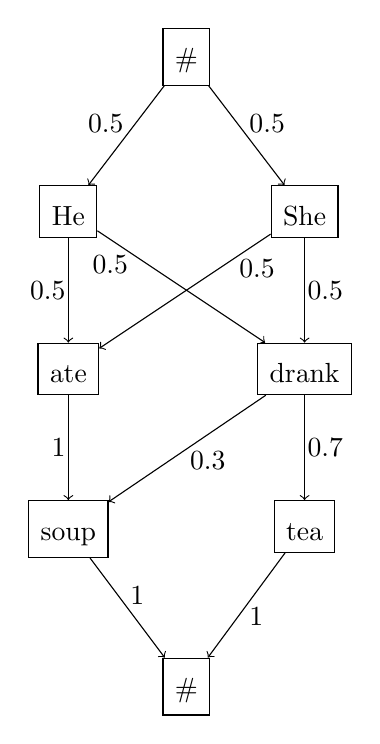
\begin{tikzpicture}[baseline=(current bounding box.north)]
   \begin{scope}[every node/.style={rectangle,draw,text height=1.0em,inner sep=1ex,anchor=north}]
    \node (v0) at (1.5,2) {\#};
    \node (v11) at (0,0) {He};
    \node (v12) at (3,0) {She};
    \node (v21) at (0,-2) {ate};
    \node (v22) at (3,-2) {drank};
    \node (v31) at (0,-4) {soup};
    \node (v32) at (3,-4) {tea};
    \node (v4) at (1.5,-6) {\#};
   \end{scope}
   \begin{scope}[every node/.style={rectangle,inner sep=0.2ex}]
    \draw[->] (v0) -- node[auto,swap] {$0.5$} (v11);
    \draw[->] (v0) -- node[auto] {$0.5$} (v12);
    \draw[->] (v11) -- node[auto,swap] {$0.5$} (v21);
    \draw[->] (v12) -- node[auto,pos=0.2] {$0.5$} (v21);
    \draw[->] (v11) -- node[auto,pos=0.2,swap] {$0.5$} (v22);
    \draw[->] (v12) -- node[auto] {$0.5$} (v22);
    \draw[->] (v21) -- node[auto,swap] {$1$} (v31);
    \draw[->] (v22) -- node[auto] {$0.3$} (v31);
    \draw[->] (v22) -- node[auto] {$0.7$} (v32);
    \draw[->] (v31) -- node[auto] {$1$} (v4);
    \draw[->] (v32) -- node[auto] {$1$} (v4);
   \end{scope}
  \end{tikzpicture}
  &&
  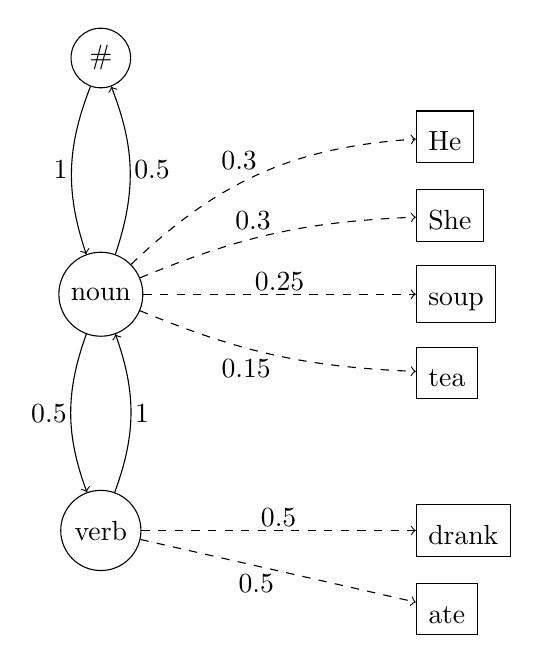
\begin{tikzpicture}[baseline=(current bounding box.north)]
   \begin{scope}[every node/.style={circle,draw}]
    \node (q0) at (0,6) {\#};
    \node (q1) at (0,3) {noun};
    \node (q2) at (0,0) {verb};
   \end{scope}
   \begin{scope}[every node/.style={rectangle,draw,text height=1.0em,inner sep=1ex,anchor=west}]
    \node (v11) at (4,5) {He};
    \node (v12) at (4,4) {She};
    \node (v13) at (4,3) {soup};
    \node (v14) at (4,2) {tea};
    \node (v21) at (4,0) {drank};
    \node (v22) at (4,-1) {ate};
   \end{scope}
   \begin{scope}[every node/.style={rectangle,inner sep=0.3ex}]
    \draw[->] (q0) edge[bend right=20] node[auto,swap] {$1$} (q1);
    \draw[->] (q1) edge[bend right=20] node[auto,swap] {$0.5$} (q2);
    \draw[->] (q1) edge[bend right=20] node[auto,swap] {$0.5$} (q0);
    \draw[->] (q2) edge[bend right=20] node[auto,swap] {$1$} (q1);
    \draw[dashed,->] (q1) edge[bend left=20] node[auto] {$0.3$} (v11);
    \draw[dashed,->] (q1) edge[bend left=10] node[auto] {$0.3$} (v12);
    \draw[dashed,->] (q1) edge node[auto] {$0.25$} (v13);
    \draw[dashed,->] (q1) edge[bend right=10] node[auto,swap] {$0.15$} (v14);
    \draw[dashed,->] (q2) edge node[auto] {$0.5$} (v21);
    \draw[dashed,->] (q2) edge node[auto,swap] {$0.5$} (v22);
   \end{scope}
  \end{tikzpicture}
 \end{align*}
\end{figure}

A further generalization of N-gram models leads to the \emph{Hidden Markov
model}. In this model, the emission probability of a word depends not on the
previous words, but on the progression of a state machine that is not visible
from the outside.  Every time a word needs to be emitted, the state machine
progresses to a new state according to a transition probability distribution
$t$ dependent on the previous state, and the next word is predicted by an
emission probability distribution $e$ dependent on the new state. The symbol
$\#$ is used as the start and end state of the state machine.
For example, if the state sequence that generated the sentence ``He ate soup''
was ``noun-verb-noun'', then the probability of that sentence would be
\begin{align*}
 p
  =&\; t(\text{noun}|\#) \cdot e(\text{He}|\text{noun}) \cdot t(\text{verb}|\text{noun}) \cdot e(\text{ate}|\text{verb}) \\
  &\cdot t(\text{noun}|\text{verb}) \cdot e(\text{soup}|\text{noun}) \cdot t(\#|\text{noun}).
\end{align*}

Since the state sequence is typically not known, the sum over all possible
state sequences must be computed. Therefore,
\[
 p(v=v_1\cdots v_n) = \sum_{q_1,\ldots,q_n} t(q_1|\#) \cdot e(v_1|q_1) \cdot \prod_{i=2}^n \mbig\brk{t(q_i|q_{i-1}) \cdot e(v_i|q_i)} \cdot t(\#|q_n).
\]

N-gram models can be interpreted a special case of the Hidden Markov model, by
using the state space $Q = V^n$ and defining the transmission and emission
probability in terms of the N-gram probability. For example, for bigrams:
\begin{align*}
 t(v_1v_2|v_1'v_2') &:= \begin{cases}
  b(v_2|v_1) & \text{if } v_1 = v_2', \\
  0 &\text{otherwise},
 \end{cases} &
 e(v|v_1v_2) &:= \begin{cases}
  1 & \text{if } v = v_2, \\
  0 &\text{otherwise}.
 \end{cases}
\end{align*}

\section{Outlook}

Many training algorithms for language models are instances of the
\emph{expectation-maximization (EM) algorithm}. \cite{demlairub77} Chapter 2
will introduce a general framework for EM algorithms that first appeared in
\cite{bucstuvog15}.

Following the short motivation above, chapter 3 will define Hidden Markov
models more formally, and discuss algorithms that act on them. Chapter 4 will
specifically focus on the standard training algorithm for Hidden Markov models,
the \emph{Baum-Welch algorithm}, in order to show that it is an instance of the
general EM algorithms laid out in chapter 2.
